\section{线性谐振子}\label{section linear oscillator}



\begin{quotation}
``要真正懂得我们在这个世界所看到的几乎所有现象背后,
自然到底在干什么,我们非违背常识不可。''\qquad 费曼
\end{quotation}


线性谐振子(Linear Oscillator)问题是很重要的问题,
以致有人说物理学家其实只会处理线性谐振子问题,
比线性谐振子更复杂的问题物理学家都不研究。(1)我们可以把线性谐振子问题看作是个微分方程求解的问题,
解出来是厄米多项式(Hermite
Polynomials)。(2)我们也可用代数法求解,
这个我们将在后面的章节中介绍。

线性谐振子的势函数:$V(x) = \frac{1}{2}m\omega ^2 x^2
$,可描述:双原子分子振动、晶格振动(声子)、电磁辐射(光子)等。
固体中原子的振动:考虑一维原子链,某原子在平衡位置附近的运动,$\Delta
x \ll a$($a$为原子最近邻间距。)

\index{Linear Oscillator: 线性谐振子}

\begin{figure}[h]
\begin{center}
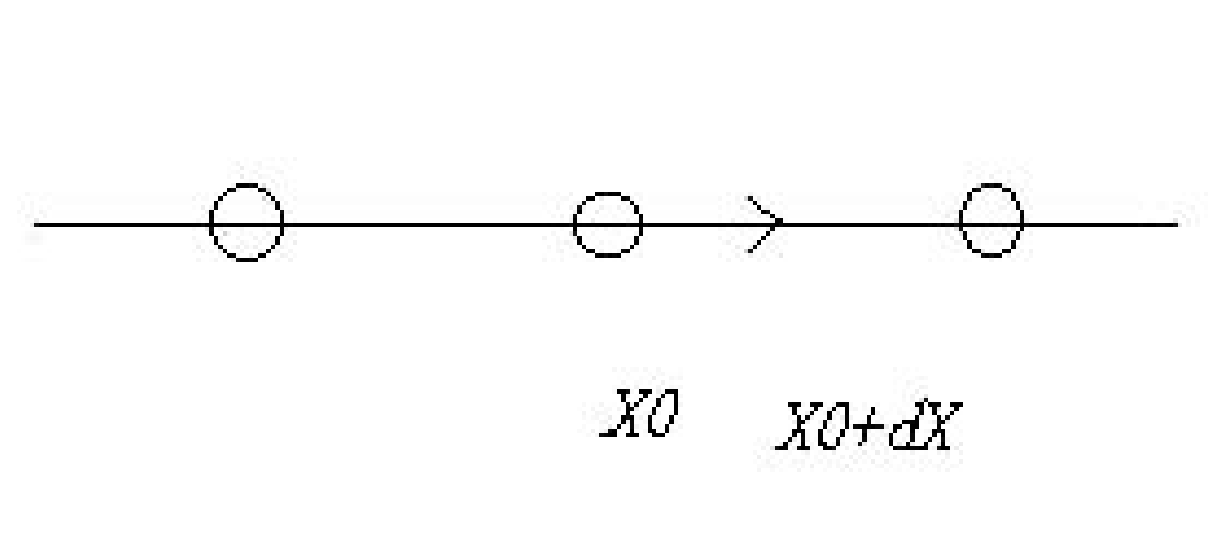
\includegraphics[clip,width=6cm]{1DProblem/10-1.ps}
\caption{原子在平衡位置附近振动。}
\end{center}
\end{figure}


原子势能在平衡位置$x_0$附近可按泰勒级数展开:

\begin{equation}
U(x) = U(x_0 ) + \left. {\frac{{\partial U}}{{\partial x}}} \right|_{x_0 } \Delta x + \left. {\frac{1}{2}\frac{{\partial ^2 U}}{{\partial x^2 }}} \right|_{x_0 } \Delta x^2  + ...
\end{equation}

$x_0$是平衡位置,满足:$\left. {\frac{{\partial U}}{{\partial x}}} \right|_{x_0 }  = 0,\left. {\frac{{\partial ^2 U}}{{\partial x^2 }}} \right|_{x_0 }  > 0$。弹性系数可定义为:

\begin{equation}
k = \frac{{\partial ^2 U}}{{\partial x^2 }} = m\omega ^2 
\end{equation}

原子的总哈密顿量可写为:

\begin{equation}\label{10-1}
H = \frac{{p^2 }}{{2m}} + \frac{1}{2}m\omega ^2 x^2
\end{equation}

$U(x)$展开式中第一项$U(x_0)$是常数,可从哈密顿量\ref{10-1}中略去不写。



\subsection{经典情形}
根据经典力学的哈密顿理论\footnote{参考:金尚年等编《理论力学》第8章},正则方程可写为:

\begin{equation}\label{10-2}
\left\{ \begin{array}{l}
 \dot x = \frac{{\partial H}}{{\partial p}} = \frac{p}{m} \\
 \dot p =  - \frac{{\partial H}}{{\partial x}} =  - m\omega ^2 x \\
 \end{array} \right.
\end{equation}

所以:$p = m\dot x$,$\dot p = m\ddot x =  - m\omega ^2 x$

得到运动方程:$m\ddot x + m\omega ^2 x = 0$,即:$\ddot x + \omega ^2 x = 0$

解的一般形式为:$x = A\sin \left( {\omega t + \delta } \right)$,这里$A$为振幅,$\delta$为初位相。不妨设:$\delta=0$,则有:

\begin{center}
$\left\{ \begin{array}{l}
 x = A\sin \omega t \\
 \dot x = \omega A\cos \omega t \\
 \ddot x =  - \omega ^2 A\sin \omega t \\
 \end{array} \right.$
\end{center}

所以能量为:

\begin{center}
$
\left\{ \begin{array}{l}
 T = {\textstyle{1 \over 2}}m\dot x^2  = {\textstyle{1 \over 2}}m\omega ^2 A^2 \cos ^2 \omega t \\
 V = {\textstyle{1 \over 2}}m\omega ^2 x^2  = {\textstyle{1 \over 2}}m\omega ^2 A^2 \sin ^2 \omega t \\
 E = T + V = {\textstyle{1 \over 2}}m\omega ^2 A^2  \\
 \end{array} \right.
$
\end{center}

振幅$A$与总能量的关系:$A = \sqrt {\frac{{2E}}{{m\omega ^2 }}} $。可见在经典情形下,能量取值范围为从零到无穷大,振幅相应为从零到无穷大。

粒子在位置$x$处的几率为:$w(x)dx = \frac{{dt}}{{T/2}}$,这里$T = \frac{{2\pi }}{\omega }$是振动周期。
所以:

$w(x)dx = \frac{{2\omega }}{{2\pi }}dt = \frac{\omega }{\pi }\frac{{dt}}{{dx}}dx = \frac{\omega }{\pi }\frac{{dx}}{{\dot x}} = \frac{\omega }{\pi }\frac{{dx}}{{\omega A\cos \omega t}} = \frac{{dx}}{{\pi A\cos \omega t}} = \frac{{dx}}{{\pi A\sqrt {1 - \left( {{\raise0.5ex\hbox{$\scriptstyle x$}
\kern-0.1em/\kern-0.15em
\lower0.25ex\hbox{$\scriptstyle A$}}} \right)^2 } }}$

经典情形下,几率密度为:$w(x) = \frac{1}{{\pi A\sqrt {1 - \left( {{\raise0.5ex\hbox{$\scriptstyle x$}
\kern-0.1em/\kern-0.15em
\lower0.25ex\hbox{$\scriptstyle A$}}} \right)^2 } }}$

可见经典情形下粒子出现几率密度分布呈U形,
粒子在平衡位置附近几率密度最小,在最大振幅处($ \pm A$)几率密度最大(趋于无穷大)。


\subsection{量子情形}

\subsubsection{利用不确定关系估算}

\index{Uncertainty principle: 不确定原理}

但在进入复杂的数学运算之前,我们先用不确定关系(uncertainty
relation)来估算一下线性谐振子的基态能(ground state energy)。

由$H = \frac{p^2}{2m} + \frac{m \omega^2 x^2}{2}$出发,利用:$a^2
+b^2 \ge 2ab$

能量:$E = \frac{(\Delta p)^2}{2m} + \frac{m \omega^2 (\Delta
x)^2}{2} \ge \frac{\omega (\Delta x) (\Delta p)}{2}$

对比严格形式的不确定关系(证明在后面章节中介绍):$\Delta x \Delta p
\ge \frac{\hbar}{2}$

有:$E \ge \frac{\omega}{2} (\Delta x) (\Delta p) \ge \frac{\hbar
\omega}{4}$

更细致的估算是假设位置的不确定度为$\Delta x
=a$,由不确定关系,得到$\Delta p = \frac{\hbar}{2a}$,那么:$ E =
\frac{\hbar^2}{8ma^2} + \frac{m \omega^2 a^2}{2}$,
为估算$E$的最小值,计算微分:$\frac{d E}{d a} = -
\frac{\hbar^2}{4ma^3} +m \omega^2 a =0$. 解出:$a^4 =
\frac{\hbar^2}{4m^2 \omega^2}$. 即:$a^2 = \frac{\hbar}{2 m
\omega}$.代入$E$的表达式中,得到:$E = \frac{\hbar \omega}{2}$。

这个估算说明在量子力学中,谐振子势中粒子的基态将不是静止在“弹簧”的平衡位置,而是存在着零点振动($\Delta
p \ne 0$),或零点能的。严格的求解表明,谐振子能级为:$E_n =(
n+\frac{1}{2} ) \hbar \omega$,$n=0,1,2,...$。

\subsubsection{定性的讨论}

在不涉及数学细节的情况下,我们仍能对线性谐振子的解做一定性讨论。


\begin{figure}[h]
\begin{center}
\includegraphics[clip,width=11cm]{1DProblem/HarmonicOscillator.ps}
\caption{线性谐振子波函数的定性行为}
\end{center}
\end{figure}


\begin{enumerate}
  \item $E<0$的解不存在。
  \item $E>0$ 的解可分为三个区域讨论,左侧$V>E$,中间$E>V$,右侧$V>E$。
  \item 对左右两侧$V>E$, 解的形式类似$e$指数形, 只是其发散或收敛指数因$V(x)$的不同而处处不同, 但由于$V(x)$是平滑的,所以波函数也应是平滑的。
  \item 中间 $E>V$,解的形式是类似正弦余弦形的(当然不严格是),能量最低的一个解,波函数振荡的形状应是最舒缓的,因此是个振荡最少的偶函数,节点数为0,对应$\psi_0$的样子。
  \item 由于$V$是平滑的,我们还要求三个区域的波函数能平滑地连接起来。
  \item 对于$V$而言,左右$V>E$的两区域总是存在的($x \to \pm \infty$ , $V(x) \to \infty$),由此可证明解是分立的。即假设$E$是薛定谔方程的解,$E$的邻域不可能是薛定谔方程的解\footnote{参考:J J Sakurai, \textbf{Modern Quantum Mechanics}, pp99. ``We know from the theory of partial differential equations that time-independent wave equation subject to boundary condition ($x \to \infty$, $\psi \to 0$) allows for nontrivial solutions only for a descrete set of values of $E$.''}。
  \item 能量次低的解是奇函数,对应$\psi_1$的样子,振荡更剧烈一些,波函数穿过横轴一次,节点数为1,能量更高的解可依此类推。
\end{enumerate}


\subsubsection{严格求解}

量子力学下,哈密顿量\ref{10-1}表示为:

\begin{equation}\label{10-3}
\hat H =  - \frac{{\hbar ^2 }}{{2m}}\frac{{d^2 }}{{dx^2 }} + \frac{{m\omega ^2 x^2 }}{2}
\end{equation}

V(x)不含t,哈密顿\ref{10-3}可表示为定态薛定谔方程的形式:

\begin{equation}\label{10-4}
 - \frac{{\hbar ^2 }}{{2m}}\frac{{d^2 }}{{dx^2 }}\psi (x) + \frac{{m\omega ^2 x^2 }}{2}\psi (x) = E\psi (x)
\end{equation}

在方程两边同时乘以$\frac{2}{{\hbar \omega }}$:

\begin{center}
$\frac{2}{{\hbar \omega }} \cdot \frac{{\hbar ^2 }}{{2m}}\psi ''(x) + \frac{2}{{\hbar \omega }} \cdot \left( {E - \frac{{m\omega ^2 x^2 }}{2}} \right)\psi (x) = 0$
\end{center}

得到:$\frac{\hbar }{{m\omega }}\psi ''(x) + \left( {\frac{{2E}}{{\hbar \omega }} - \frac{{m\omega x^2 }}{\hbar }} \right)\psi (x) = 0$,定义:$\alpha  = \sqrt {\frac{{m\omega }}{\hbar }} $,$\lambda  = \frac{{2E}}{{\hbar \omega }}$

得到:$\frac{1}{{\alpha ^2 }}\psi ''(x) + \left( {\lambda  - \alpha ^2 x^2 } \right)\psi (x) = 0$

引入无量纲变量:$\xi  = x\sqrt {\frac{{m\omega }}{\hbar }}  = \alpha x,\alpha  = \sqrt {\frac{{m\omega }}{\hbar }} $;则:$d\xi  = \alpha dx,d\xi ^2  = \alpha ^2 dx^2 $。

方程可改写为:

\begin{equation}\label{10-5}
\frac{{d^2 \psi (\xi )}}{{d\xi ^2 }} + \left( {\lambda  - \xi ^2 } \right)\psi (\xi ) = 0
\end{equation}

对方程\ref{10-5}定性讨论:

\begin{enumerate}
    \item $\xi  \to  \pm \infty ,V \to \infty ,\left| \psi  \right| \to 0$,$\frac{{d^2 \psi (\xi )}}{{d\xi ^2 }} = \xi ^2 \psi (\xi )$,$\psi  \sim \exp \left( { - {\textstyle{1 \over 2}}\xi ^2 } \right)$,为指数型衰减;
    \item $\xi  \to 0,V \to 0$,$\psi$应为正弦($\sin$)或余弦($\cos$)型的。
   \end{enumerate}


\begin{figure}[h]
\begin{center}
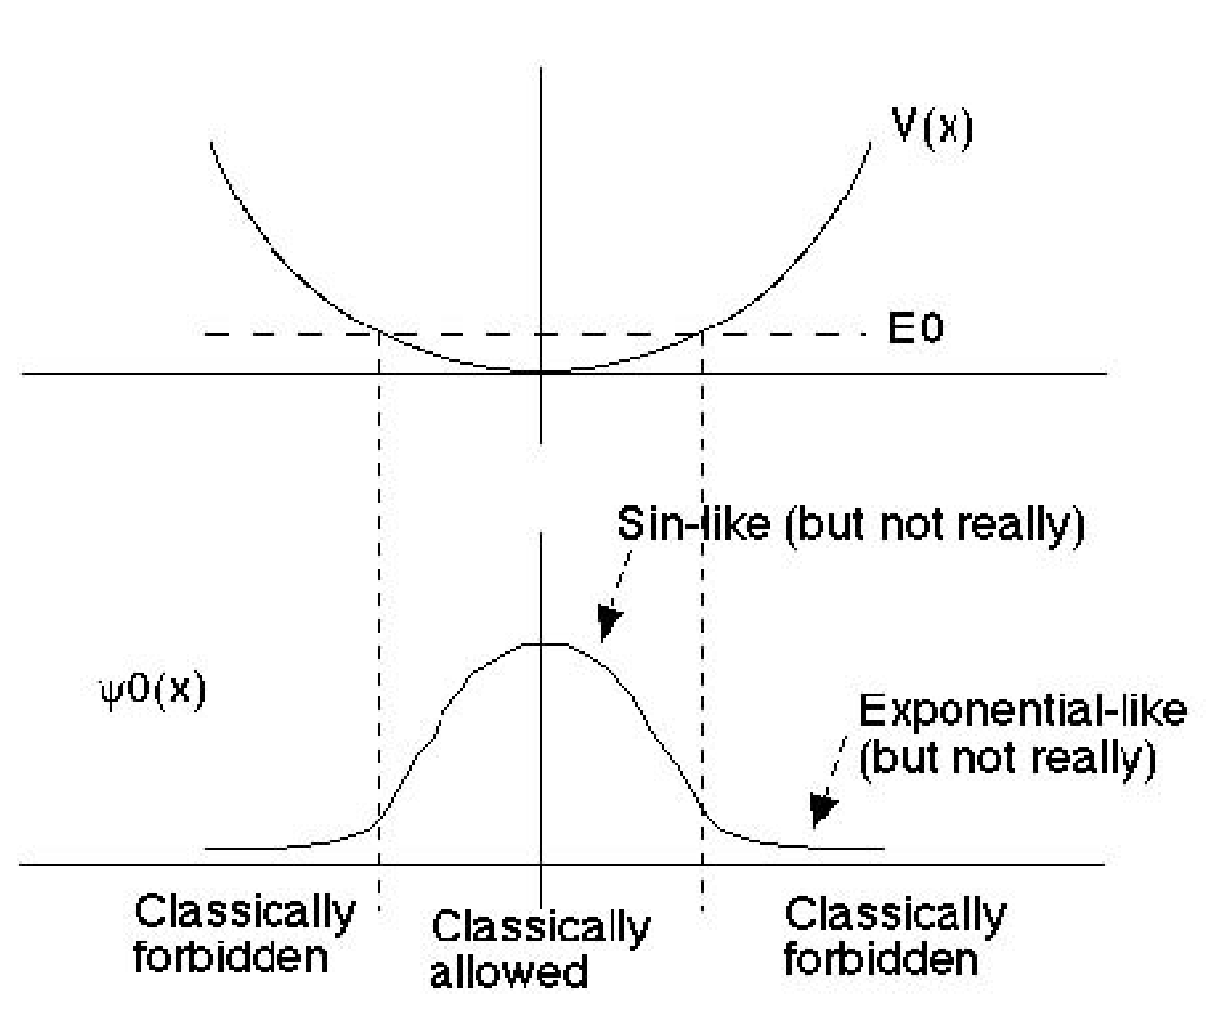
\includegraphics[clip,width=8cm]{1DProblem/10-3.ps}
\caption{线性谐振子基态波函数的定性行为}
\end{center}
\end{figure}


基于以上分析,我们把待求波函数解表示为:$\psi (\xi ) = e^{ - \frac{{\xi ^2 }}{2}} H\left( \xi  \right)$,所以:

\begin{eqnarray*}
\frac{{d\psi }}{{d\xi }} & =  &  - \xi e^{ - {\textstyle{{\xi ^2 } \over 2}}} H\left( \xi  \right) + e^{ - {\textstyle{{\xi ^2 } \over 2}}} \frac{{dH\left( \xi  \right)}}{{d\xi }} = \left( { - \xi H + H'} \right)e^{ - {\textstyle{{\xi ^2 } \over 2}}} \\
 \frac{{d^2 \psi }}{{d\xi ^2 }} & = & \left( { - H - \xi H' + H''} \right)e^{ - \frac{{\xi ^2 }}{2}}  - \xi \left( { - \xi H + H'} \right)e^{ - \frac{{\xi ^2 }}{2}} \\
 {} & = & \left( { - H + \xi ^2 H - 2\xi H' + H''} \right)e^{ - \frac{{\xi ^2 }}{2}}
\end{eqnarray*}

所以:

\begin{equation*}
\left( { - H + \xi ^2 H - 2\xi H' + H''} \right)e^{ - \frac{{\xi ^2 }}{2}}  + \left( {\lambda H - \xi ^2 H} \right)e^{ - \frac{{\xi ^2 }}{2}}  = 0
\end{equation*}

即:

\begin{equation}\label{10-6}
H'' - 2\xi H' + \left( {\lambda  - 1} \right)H = 0
\end{equation}

常微分方程\ref{10-6}称为厄密方程\footnote{参考:梁昆淼编《数学物理方法》第487页},可用级数解法求解,令:$H\left( \xi  \right) = \sum\limits_{\nu  = 0}^\infty  {a_\nu  \xi ^\nu  } $


\begin{center}
$\begin{array}{l}
 H'\left( \xi  \right) = a_1  + 2a_2 \xi  + ... + \left( {\nu  + 1} \right)a_{\nu  + 1} \xi ^\nu   + ... \\
 H''\left( \xi  \right) = 2a_2  + 6a_3 \xi  + ... + \left( {\nu  + 2} \right)\left( {\nu  + 1} \right)a_{\nu  + 2} \xi ^\nu   + ... \\
 \end{array}$
\end{center}

方程\ref{10-6}化为:

\begin{center}
$\begin{array}{l}
 2a_2  + 6a_3 \xi  + ... + \left( {\nu  + 2} \right)\left( {\nu  + 1} \right)a_{\nu  + 2} \xi ^\nu   + ... \\
  - 2\xi \left[ {a_1  + 2a_2 \xi  + ... + \left( {\nu  + 1} \right)a_{\nu  + 1} \xi ^\nu   + ...} \right] \\
  + \left( {\lambda  - 1} \right)\sum\limits_{\nu  = 0}^\infty  {a_\nu  \xi ^\nu  }  = 0 \\
 \end{array}$
\end{center}

考虑含$\xi ^\nu$的项:

\begin{center}
$\xi ^\nu  \left[ {\left( {\nu  + 2} \right)\left( {\nu  + 1} \right)a_{\nu  + 2}  - 2\nu a_\nu   + \left( {\lambda  - 1} \right)a_\nu  } \right] = 0$
\end{center}

可得到关系:

\begin{equation}\label{10-7}
a_{_{\nu  + 2} }  = \frac{{2\nu  - \lambda  + 1}}{{\left( {\nu  + 2} \right)\left( {\nu  + 1} \right)}}a_\nu
\end{equation}


如已知$a_0$、$a_1$,根据关系\ref{10-7}可分别计算出所有含$\xi ^\nu$偶数幂项和含$\xi ^\nu$奇数幂项的系数。



假设级数展开包括无穷项,则:$\nu  \to \infty  \Rightarrow \frac{{a_{\nu  + 2} }}{{a_\nu  }} = \frac{{2\nu  - \lambda  + 1}}{{\left( {\nu  + 2} \right)\left( {\nu  + 1} \right)}} \to \frac{2}{\nu }$

由于:$e^{\xi ^2 }  = 1 + \frac{{\xi ^2 }}{{1!}} + \frac{{\xi ^4 }}{{2!}} + ... + \frac{{\xi ^\nu  }}{{\left( {{\textstyle{\nu  \over 2}}} \right)!}} + \frac{{\xi ^{\nu  + 2} }}{{\left( {{\textstyle{\nu  \over 2}} + 1} \right)!}} + ...$

其系数之比在$\nu  \to \infty $时:$\frac{{\left( {{\textstyle{\nu  \over 2}}} \right)!}}{{\left( {{\textstyle{\nu  \over 2}} + 1} \right)!}} = \frac{1}{{\left( {{\textstyle{\nu  \over 2}} + 1} \right)}} \to \frac{2}{\nu }$

可见若$H(\xi )$包含无穷项,其在$\xi  \to \infty $时,发散速度与$e^{\xi ^2 } $相同,由波函数的定义:$\psi (\xi ) = e^{ - \frac{{\xi ^2 }}{2}} H\left( \xi  \right)$,$\left| \psi  \right| \propto e^{{\textstyle{{\xi ^2 } \over 2}}}  \to \infty $,这是不可以的。

因此$H(\xi )$的级数展开只能包含有限项,即可展开为多项式的形式。

如:$\lambda  = 2n + 1$,则$a_n  \ne 0$,$a_{n + 2}  = a_{n + 4}  = ... = 0$。

同时令:$a_0  = 0$(即全部偶数项系数为0),或$a_1  = 0$(即全部奇数项系数为0),可保证$a_{n + 1}  = a_{n + 3}  = ... = 0$,这样对确定本征值$\lambda  = 2n + 1$,$H(\xi )$最多只能展开到第n项,记作$H_n (\xi )$,称为厄密多项式(Hermite Polynomials)。$H_n (\xi )$满足公式:

\begin{equation}\label{10-8}
\frac{{d^2 H_n }}{{d\xi ^2 }} - 2\xi \frac{{dH_n }}{{d\xi }} + 2nH_n  = 0
\end{equation}

由于$H_n (\xi )$只含有$\xi ^\nu  $的奇次幂或偶次幂,$H_n (\xi )$有确定的奇偶性,$H_n ( - \xi ) = \left( { - 1} \right)^n H_n (\xi )$,所以:$\psi _n ( - x) = \left( { - 1} \right)^n \psi _n (x)$(n偶,偶宇称,n奇,奇宇称;)


由$\lambda  = 2n + 1 = \frac{{2E}}{{\hbar \omega }}$,得到能量本征值:

\begin{equation}\label{10-8}
E_n  = \left( {n + {\textstyle{1 \over 2}}} \right)\hbar \omega, (n = 0,1,2...)
\end{equation}


厄密多项式的微分表示式为\footnote{令:$u = e^{ - \xi ^2 } ,\frac{{du}}{{d\xi }} =  - 2\xi u$, 则:$\frac{{d^{n + 2} u}}{{d\xi ^{n + 2} }} =  - 2\xi \frac{{d^{n + 1} u}}{{d\xi ^{n + 1} }} - 2(n + 1)\frac{{d^n u}}{{d\xi ^n }}$。

若:$\frac{{d^n u}}{{d\xi ^n }} = \left( { - 1} \right)^n e^{ - \xi ^2 } H_n \left( \xi  \right)$

则:$\frac{{d^{n + 1} u}}{{d\xi ^{n + 1} }} = ( - 1)^n ( - 2\xi )e^{ - \xi ^2 } H_n  + ( - 1)^n e^{ - \xi ^2 } H'_n $

所以:$\frac{{d^{n + 2} u}}{{d\xi ^{n + 2} }} =  - 2\left( { - 1} \right)^n \left( {e^{ - \xi ^2 }  + \xi \left( { - 2\xi } \right)e^{ - \xi ^2 } } \right)H_n  + \left( { - 1} \right)^n \left( { - 2\xi } \right)e^{ - \xi ^2 } H'_n  + \left( { - 1} \right)^n \left( { - 2\xi } \right)e^{ - \xi ^2 } H'_n  + \left( { - 1} \right)^n e^{ - \xi ^2 } H''_n $

化简后:$H''_n  - 2\xi H'_n  + 2nH_n  = 0$,即:$H_n \left( \xi  \right) = \left( { - 1} \right)^n e^{\xi ^2 } \frac{{d^n }}{{d\xi ^n }}e^{ - \xi ^2 } $满足这个微分方程。

所以厄密多项式可表示为:$H_n \left( \xi  \right) = \left( { - 1} \right)^n e^{\xi ^2 } \frac{{d^n }}{{d\xi ^n }}e^{ - \xi ^2 } $}:

\begin{center}
$H_n \left( \xi  \right) = \left( { - 1} \right)^n e^{\xi ^2 } \frac{{d^n }}{{d\xi ^n }}e^{ - \xi ^2 } $
\end{center}

厄密多项式$H_n (\xi )$还满足递推关系:

\begin{center}
$H_{n + 2} \left( \xi  \right) - 2\xi H_{n + 1} \left( \xi  \right) + 2(n + 1)H_n \left( \xi  \right) = 0$
\end{center}

波函数用厄密多项式表示:

\begin{equation*}
\psi _n (\xi ) = e^{ - \frac{{\xi ^2 }}{2}} H_n \left( \xi  \right) = e^{ - \frac{{\xi ^2 }}{2}} \left( { - 1} \right)^n e^{\xi ^2 } \frac{{d^n }}{{d\xi ^n }}e^{ - \xi ^2 },
\end{equation*}

这里$\xi  = \alpha x$。

归一化:

\begin{equation*}
\int_{ - \infty }^\infty  {\psi _n ^* (x)\psi _n (x)dx}  = \frac{{N_n ^2 }}{\alpha }\int_{ - \infty }^\infty  {\psi _n ^* (\xi )\psi _n (\xi )} d\xi  = 1
\end{equation*}

积分$\int_{ - \infty }^\infty  {\psi _n ^* (\xi )\psi _n (\xi )} d\xi $为:

\begin{center}
$\begin{array}{l}
 \int_{ - \infty }^\infty  {\psi _n ^* (\xi )\psi _n (\xi )} d\xi  = \int_{ - \infty }^\infty  {e^{ - \xi ^2 } H_n ^2 \left( \xi  \right)} d\xi  \\
  = \left( { - 1} \right)^n \int_{ - \infty }^\infty  {e^{ - \xi ^2 } H_n \left( \xi  \right)e^{\xi ^2 } \frac{{d^n \left( {e^{ - \xi ^2 } } \right)}}{{d\xi ^n }}d\xi }  = \left( { - 1} \right)^n \int_{ - \infty }^\infty  {H_n \left( \xi  \right)} \frac{{d^n \left( {e^{ - \xi ^2 } } \right)}}{{d\xi ^n }}d\xi  \\
  = \left. {\left( { - 1} \right)^n H_n \left( \xi  \right)\frac{{d^{n - 1} e^{ - \xi ^2 } }}{{d\xi ^{n - 1} }}} \right|_{ - \infty }^\infty   + \left( { - 1} \right)^{n + 1} \int_{ - \infty }^\infty  {\frac{{dH_n \left( \xi  \right)}}{{d\xi }}\frac{{d^{n - 1} e^{ - \xi ^2 } }}{{d\xi ^{n - 1} }}d\xi }  = 0 + ... \\
  = \left( { - 1} \right)^{2n} \int_{ - \infty }^\infty  {\frac{{d^n H_n \left( \xi  \right)}}{{d\xi ^n }}}  \cdot e^{ - \xi ^2 } d\xi  = \left( { - 1} \right)^{2n} 2^n n!\int_{ - \infty }^\infty  {e^{ - \xi ^2 } d\xi }  = 2^n n!\sqrt \pi   \\
 \end{array}$
\end{center}

归一化常数:$N_n  = \left( {\frac{\alpha }{{2^n n!\sqrt \pi  }}} \right)^{1/2} $

归一化波函数为:$\psi _n (x) = N_n e^{ - {\textstyle{{\alpha ^2 x^2 } \over 2}}} H_n \left( {\alpha x} \right)$

最低级的几个厄密多项式为:

\index{Hermite Polynomials: 厄米多项式}

\begin{center}
$
\left\{ \begin{array}{l}
 H_0 (\xi ) = 1 \\
 H_1 (\xi ) = 2\xi  \\
 H_2 (\xi ) = 4\xi ^2  - 2 \\
 H_3 (\xi ) = 8\xi ^3  - 12\xi  \\
 ... \\
 \end{array} \right.
$
\end{center}

相应最低级的几个谐振子波函数为:


\begin{center}
$
\left\{ \begin{array}{l}
 \psi _0 (x) = \left( {\frac{\alpha }{{\sqrt \pi  }}} \right)^{1/2} e^{ - \frac{{\alpha ^2 x^2 }}{2}}  \\
 \psi _1 (x) = \left( {\frac{{2\alpha }}{{\sqrt \pi  }}} \right)^{1/2} \alpha xe^{ - \frac{{\alpha ^2 x^2 }}{2}}  \\
 \psi _2 (x) = \left( {\frac{\alpha }{{2\sqrt \pi  }}} \right)^{1/2} \left( {2\alpha ^2 x^2  - 1} \right)e^{ - \frac{{\alpha ^2 x^2 }}{2}}  \\
 \psi _3 (x) = \left( {\frac{{3\alpha }}{{\sqrt \pi  }}} \right)^{1/2} \alpha x\left( {\frac{2}{3}\alpha ^2 x^2  - 1} \right)e^{ - \frac{{\alpha ^2 x^2 }}{2}}  \\
 ... \\
 \end{array} \right.
$
\end{center}



\subsection{讨论}

\begin{figure}[h]
\begin{center}
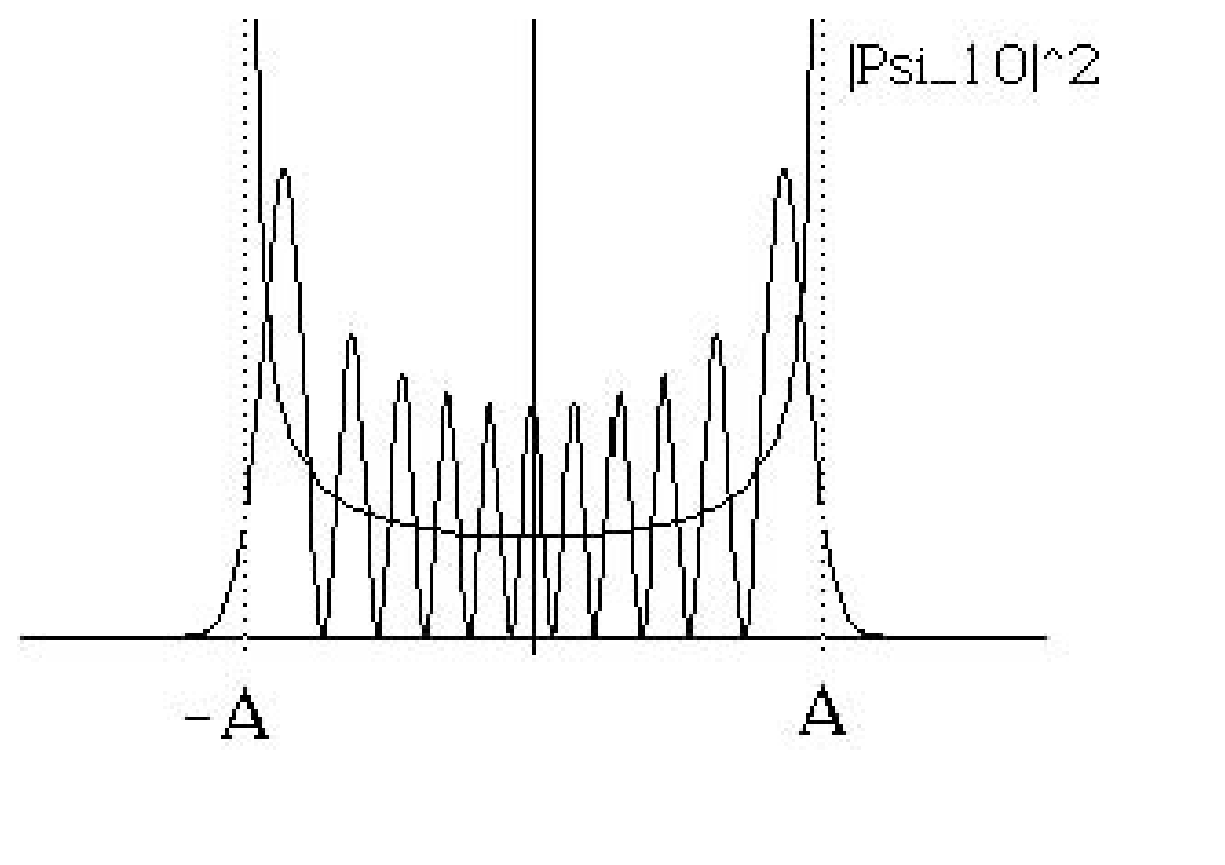
\includegraphics[clip,width=8cm]{1DProblem/10-2.ps}
\caption{一维谐振子粒子出现几率密度分布,经典与量子情形的比较}
\end{center}
\end{figure}


\begin{enumerate}
    \item 谐振子能量量子化,$E_{n + 1}  - E_n  = \hbar \omega $,与普郎克假设一致;

    \item 基态能不为0,$E_0  = {\textstyle{1 \over 2}}\hbar \omega $,称为零点能。零点能可用不确定原理说明:

$\bar x = 0,\bar p = 0$,$\left\{ \begin{array}{l}
 \overline {\Delta p^2 }  = \overline {\left( {p - \bar p} \right)^2 }  = \overline {p^2 }  - \bar p^2  = \overline {p^2 }  \\
 \overline {\Delta x^2 }  = \overline {\left( {x - \bar x} \right)^2 }  = \overline {x^2 }  - \bar x^2  = \overline {x^2 }  \\
 \end{array} \right.$

由不确定关系:$\overline {p^2 }  \cdot \overline {x^2 }  \ge \frac{{\hbar ^2 }}{4} \Rightarrow \overline {x^2 }  \ge \frac{{\hbar ^2 }}{{4\overline {p^2 } }}$

所以:$\bar H = \overline {\frac{{p^2 }}{{2m}} + \frac{{m\omega ^2 x^2 }}{2}}  = \frac{{\overline {p^2 } }}{{2m}} + \frac{{m\omega ^2 }}{2}\overline {x^2 }  \ge \frac{{\overline {p^2 } }}{{2m}} + \frac{{m\omega ^2 }}{2}\frac{{\hbar ^2 }}{{4\overline {p^2 } }} \ge 2\sqrt {\frac{{m\omega ^2 \hbar ^2 }}{{16m}}}  = \frac{1}{2}\hbar \omega $

即不确定原理要求最小能量为${\textstyle{1 \over 2}}\hbar \omega $。

    \item 几率密度:以基态为例,归一化波函数:$\psi _0  = \left( {\frac{\alpha }{{\sqrt \pi  }}} \right)^{1/2} e^{ - \frac{{\alpha ^2 x^2 }}{2}} $

$w\left( x \right)dx = \left| {\psi _0 \left( x \right)} \right|^2 dx = \frac{\alpha }{{\sqrt \pi  }}e^{ - \alpha ^2 x^2 } $,几率密度最大值出现在$x=0$处,这与经典情形是截然不同的。

当$n \to \infty $,量子情形与经典情形逐渐接近,
区别在于量子情形几率密度$\left| {\psi _n } \right|^2 $是迅速振荡的,
而经典情形则是一平滑曲线,就其平均效果而言
\footnote{$n \to \infty $时,几率密度振荡速度趋于无穷,
我们作任何经典意义上的物理测量都依赖于具体的物理仪器或物理过程,
其``反应速度''不可能是无穷快的,因此我们只能获得平均意义上的测量结果。},
当$n \to \infty $时,量子情形趋于经典情形。

    \item 量子情形时,粒子可出现在能量小于势能的区域,这是经典情形不允许的。粒子在能量E小于势垒高度时仍能出现的现象,称为隧道效应。
   \end{enumerate}


